\documentclass[12pt,a4paper]{report}

\usepackage[margin=1in]{geometry}
\usepackage[T1]{fontenc}
\usepackage[utf8]{inputenc}
\usepackage{amsmath,amssymb,amsthm}
\usepackage{booktabs}
\usepackage{array}
\usepackage{graphicx}
\usepackage{hyperref}

\hypersetup{
    colorlinks=true,
    linkcolor=blue,
    urlcolor=blue,
    citecolor=blue
}

\newtheorem{lemma}{Lemma}[chapter]
\newtheorem{theorem}{Theorem}[chapter]
\newtheorem{proposition}{Proposition}[chapter]

\title{
    \vspace{-1.5cm}
    \textbf{Primality Testing: Theory, Implementation, and Experimental Comparison}\\[0.4cm]
    \large A Project Report for CS648
}
\author{
    Group No.\ 230272
}
\date{\today}

\begin{document}

\begin{titlepage}
    \centering
    \vspace*{2.5cm}
    {\Huge \textbf{Primality Testing: Theory, Implementation, and Experimental Comparison}\par}
    \vspace{1cm}
    {\Large A Project Report for CS648\par}
    \vspace{1.5cm}
    {\Large Group No.\ 230272\par}
    \vspace{1cm}
    {\large \today\par}
    \vfill
    {\large This report presents the design, analysis, implementation, and evaluation of a primality-testing project containing a square-root baseline, Miller-Rabin primality testing with two modular reduction strategies, an AKS implementation, and a C++/Python user interface.\par}
    \vfill
\end{titlepage}

\pagenumbering{roman}
\tableofcontents
\clearpage

\chapter*{Abstract}
\addcontentsline{toc}{chapter}{Abstract}
Primality testing is a central problem in number theory and cryptography because many practical systems depend on the efficient detection of large prime numbers. This project studies primality testing from both theoretical and practical viewpoints. The codebase implements four main ideas: a simple square-root primality test, Miller-Rabin with ordinary modular reduction, Miller-Rabin with a faster modular reduction routine, and the deterministic AKS primality test. In addition, the project includes a console program, a C++ backend, a Python Tkinter graphical interface, prime generation utilities, neighbor-prime search utilities, and benchmarking scripts.

The main focus of the report is the Miller-Rabin test because it offers a strong balance between efficiency and reliability. We present the mathematical idea behind the algorithm, give a simplified correctness proof for prime inputs, and explain why repeated rounds make false acceptance of composite numbers very unlikely in the randomized version of the test. The experimental plots in the report show a clear practical pattern: Miller-Rabin remains fast even as input size grows, while AKS becomes expensive very quickly and simple methods stop being practical after relatively small bit lengths. These results confirm the common observation that probabilistic primality tests are usually the best engineering choice for large-number applications.

\clearpage
\pagenumbering{arabic}

\chapter{Introduction}
Primality testing asks whether a given positive integer is prime or composite. Although the question is simple to state, efficient solutions become nontrivial when the input is very large. This matters in several real applications, especially in public-key cryptography, where large prime numbers are needed for key generation and related arithmetic.

This project was built as a combined theory-and-implementation study of primality testing. Instead of focusing on one single algorithm, the project compares four approaches with different strengths:
\begin{itemize}
    \item the square-root method, which is exact but slow,
    \item Miller-Rabin with ordinary modulo arithmetic,
    \item Miller-Rabin with a faster modular reduction routine,
    \item and the deterministic AKS primality test.
\end{itemize}

The repository also turns these algorithms into usable software. It contains a console application for decimal and hexadecimal inputs, a backend executable that returns structured results, a Tkinter GUI for interactive use, and scripts that benchmark both individual tests and prime-search behavior across growing input sizes.

The purpose of this report is to document the mathematical background, explain the implementation choices, and summarize the experimental behavior shown by the included runtime comparisons.

\chapter{Project Objectives}
The main objectives of the project are listed below.
\begin{enumerate}
    \item Implement primality-testing algorithms with clearly different complexity and practical behavior.
    \item Build the core arithmetic needed to support large inputs through a custom \texttt{big\_int} type.
    \item Compare ordinary and faster modular reduction inside the Miller-Rabin framework.
    \item Provide both command-line and graphical interfaces for checking numbers and generating probable primes.
    \item Evaluate algorithm performance using benchmark scripts and generated CSV data.
\end{enumerate}

In short, the project is not only about deciding primality. It is also about understanding how theory, implementation details, and runtime behavior interact.

\chapter{Mathematical Background}
\section{Prime Numbers}
A prime number is an integer greater than \(1\) that has no positive divisors other than \(1\) and itself. A composite number is an integer greater than \(1\) that is not prime.

\section{Fermat's Little Theorem}
One of the classical starting points for primality testing is Fermat's Little Theorem:
\[
a^{p-1} \equiv 1 \pmod{p}
\]
for every prime \(p\) and every integer \(a\) with \(\gcd(a,p)=1\).

This theorem suggests a primality test: if a number \(n\) fails this congruence for some base \(a\), then \(n\) is certainly composite. However, the converse is not always true. Some composite numbers can still satisfy the congruence for many bases, and Carmichael numbers are the standard counterexample. Because of this weakness, a stronger test is preferred in practice.

\section{A Step-by-Step Path to Miller-Rabin}
Miller-Rabin can be understood as a sequence of improvements over Fermat's test. A direct step-by-step derivation is as follows.

\subsection{Step 1: Start with Fermat's idea}
For a prime \(p\) and any integer \(a\) with \(\gcd(a,p)=1\),
\[
a^{p-1} \equiv 1 \pmod{p}.
\]
So the first natural idea is this: given \(n\), choose a base \(a\) and check whether
\[
a^{n-1} \equiv 1 \pmod{n}.
\]
If the congruence fails, then \(n\) must be composite. This gives a simple randomized test based on repeatedly trying different bases.

\subsection{Step 2: Bases with \texorpdfstring{$\gcd(a,n)>1$}{gcd(a,n)>1} already reveal compositeness}
The next question is: which bases can possibly pass Fermat's test when \(n\) is composite? The easiest case is when \(a\) shares a factor with \(n\).

\begin{proposition}
If \(1<a<n\) and \(\gcd(a,n)>1\), then
\[
a^{n-1} \not\equiv 1 \pmod{n}.
\]
\end{proposition}

\begin{proof}
Let \(g=\gcd(a,n)\), so \(g>1\). Since \(g\mid a\), we also have \(g\mid a^{n-1}\).

Now assume for contradiction that
\[
a^{n-1} \equiv 1 \pmod{n}.
\]
Then \(n\mid (a^{n-1}-1)\), and because \(g\mid n\), it follows that \(g\mid (a^{n-1}-1)\) as well.

So \(g\) divides both \(a^{n-1}\) and \(a^{n-1}-1\). Therefore \(g\) divides their difference:
\[
a^{n-1}-(a^{n-1}-1)=1.
\]
But no integer greater than \(1\) can divide \(1\). This is a contradiction. Hence
\[
a^{n-1} \not\equiv 1 \pmod{n}.
\]
\end{proof}

This means that only bases \(a\) with \(\gcd(a,n)=1\) can possibly fool the Fermat test.

\subsection{Step 3: If one coprime base fails, many coprime bases fail}
Let \(a\) be a composite number, and let
\[
S=\{x\in\{2,3,\dots,a-1\} : \gcd(x,a)=1\}.
\]
We now use a direct proof of the same idea.

\begin{lemma}
Let \(a\) and \(p\) be coprime integers. Then for any integers \(i,j\) such that \(1\le i,j<p\) and \(i\neq j\), the following inequality holds:
\[
(a\cdot i)\bmod p \neq (a\cdot j)\bmod p.
\]
\end{lemma}

\begin{proof}
Assume, for contradiction, that
\[
(a\cdot i)\bmod p = (a\cdot j)\bmod p.
\]
Then there exist integers \(u,v\) such that
\[
a\cdot i =u\cdot p +\alpha,
\qquad
a\cdot j =v\cdot p +\beta,
\]
where \(0\le \alpha,\beta<p\) and \(\alpha=\beta\). Without loss of generality, suppose \(i>j\). Subtracting the two equations yields
\[
a\cdot (i-j) = (u-v)\cdot p.
\]
Since \(\gcd(a,p)=1\), by Bézout's identity, there exist integers \(x,y\) such that
\[
ax+py=1.
\]
Rewriting \(a\) using this identity:
\[
a=\frac{1-py}{x}.
\]
Substituting into the previous equation gives
\[
\left(\frac{1-py}{x}\right)\cdot (i-j)=(u-v)\cdot p.
\]
Rearranging and taking modulo \(p\) on both sides results in
\[
(i-j)\bmod p=0,
\]
which implies
\[
i=j \pmod p.
\]
Given that \(1\le i,j<p\), this contradicts the assumption that \(i\neq j\). Therefore, the original assumption must be false, proving the lemma:
\[
(a\cdot i)\bmod p \neq (a\cdot j)\bmod p.
\]
\end{proof}

\begin{lemma}
Let \(\gcd(a,p)=1\) and \(\gcd(b,p)=1\). Then it follows that
\[
\gcd((ab)\bmod p,p)=1.
\]
\end{lemma}

\begin{proof}
Since \(\gcd(a,p)=1\), there exist integers \(x\) and \(y\) such that
\[
ax+py=1.
\]
Similarly, since \(\gcd(b,p)=1\), there exist integers \(s\) and \(t\) such that
\[
bs+pt=1.
\]
Multiplying both equations yields
\[
(ax+py)(bs+pt)=1.
\]
Expanding the product:
\[
ab\cdot xs+p\cdot (pyt+axt+bsy)=1.
\]
Define \(V=xs\) and \(W=pyt+axt+bsy\), so we obtain
\[
ab\cdot V+p\cdot W=1.
\]
This implies that
\[
\gcd(ab,p)=1.
\]
To show \(\gcd((ab)\bmod p,p)=1\), consider the congruence
\[
ab\cdot V+p\cdot W\equiv 1 \pmod p.
\]
Since \(p\cdot W\equiv 0 \pmod p\), this implies
\[
ab\cdot V\equiv 1 \pmod p.
\]
Let \(\gamma =V\bmod p\). Then
\[
((ab)\bmod p)\cdot \gamma \equiv 1 \pmod p.
\]
This implies that \((ab)\bmod p\) has a multiplicative inverse modulo \(p\), hence
\[
\gcd((ab)\bmod p,p)=1.
\]
\end{proof}

\begin{proposition}
Let \(S\) denote the set of integers in the range \([2,a-1]\) that are coprime to \(a\). If there exists at least one element \(x_j\in S\) such that
\[
x_j^{a-1}\not\equiv 1 \pmod{a},
\]
then at least half of the elements in \(S\) also satisfy
\[
x^{a-1}\not\equiv 1 \pmod{a}.
\]
\end{proposition}

\begin{proof}
For every \(x_i\in S\), exactly one of the following conditions must hold:
\[
x_i^{a-1}\equiv 1 \pmod a
\quad \text{or} \quad
x_i^{a-1}\not\equiv 1 \pmod a.
\]
By assumption, there exists at least one element \(x_j\in S\) such that
\[
x_j^{a-1}\not\equiv 1 \pmod a.
\]

Suppose, for the sake of contradiction, that more than half of the elements in \(S\) satisfy
\[
x_i^{a-1}\equiv 1 \pmod a,
\qquad \forall x_i\in S',
\]
where
\[
S'=\{x_1,x_2,\dots,x_{\lfloor N/2\rfloor+1}\}\subseteq S.
\]

Now, construct a new set \(S''\) by multiplying each element in \(S'\) by \(x_j\), taken modulo \(a\):
\[
S''=\{(x_j\cdot x_1)\bmod a,(x_j\cdot x_2)\bmod a,\dots,(x_j\cdot x_{\lfloor N/2\rfloor+1})\bmod a\}.
\]

\begin{itemize}
    \item By Lemma 3.1, since \(\gcd(x_j,a)=1\), the mapping \(x_i\mapsto (x_j\cdot x_i)\bmod a\) is a bijection on \(S'\), so all elements in \(S''\) are distinct.
    \item By the second lemma, each product \((x_j\cdot x_i)\bmod a\) remains coprime to \(a\), that is,
    \[
    \gcd((x_j\cdot x_i)\bmod a,a)=1
    \qquad
    \forall x_i\in S'.
    \]
    Hence, all elements of \(S''\subseteq S\).
\end{itemize}

Now, consider the expression \((x_j\cdot x_i)^{a-1}\bmod a\) for any \(x_i\in S'\). By properties of modular exponentiation,
\[
(x_j\cdot x_i)^{a-1}\equiv x_j^{a-1}\cdot x_i^{a-1}\pmod a.
\]

\begin{itemize}
    \item Since \(x_i\in S'\), we have
    \[
    x_i^{a-1}\equiv 1 \pmod a
    \]
    by assumption.
    \item Therefore,
    \[
    (x_j\cdot x_i)^{a-1}\equiv x_j^{a-1}\pmod a.
    \]
    \item Given that \(x_j^{a-1}\not\equiv 1 \pmod a\), it follows that
    \[
    (x_j\cdot x_i)^{a-1}\not\equiv 1 \pmod a,
    \qquad
    \forall x_i\in S'.
    \]
\end{itemize}

This implies:
\begin{itemize}
    \item There are at least \(\lfloor N/2\rfloor+1\) distinct elements in \(S''\subseteq S\) such that
    \[
    x^{a-1}\not\equiv 1 \pmod a.
    \]
    \item By the contradiction assumption, there are also at least \(\lfloor N/2\rfloor+1\) elements in \(S\) satisfying
    \[
    x^{a-1}\equiv 1 \pmod a.
    \]
    \item These two collections are disjoint, because one collection satisfies \(x^{a-1}\equiv 1 \pmod a\) and the other satisfies \(x^{a-1}\not\equiv 1 \pmod a\).
    \item Therefore \(S\) would contain at least
    \[
    (\lfloor N/2\rfloor+1)+(\lfloor N/2\rfloor+1)>N
    \]
    elements, which is impossible.
\end{itemize}

Therefore, the initial assumption must be false. Hence, it must be true that at least half of the elements in \(S\) satisfy
\[
x^{a-1}\not\equiv 1 \pmod a.
\]
\end{proof}

So if one coprime witness exists, then many coprime witnesses exist as well.

\begin{figure}[htbp]
\centering
\begin{minipage}[t]{0.48\textwidth}
\centering
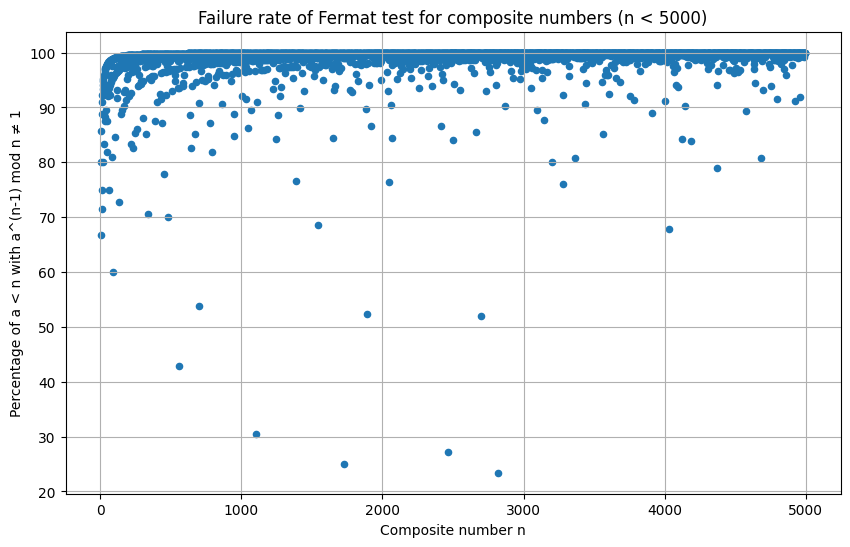
\includegraphics[width=\textwidth]{experiment_plots/failure_fermat.png}
\caption*{All bases \(a<n\): most composite numbers fail Fermat's congruence for a large majority of bases.}
\end{minipage}
\hfill
\begin{minipage}[t]{0.48\textwidth}
\centering
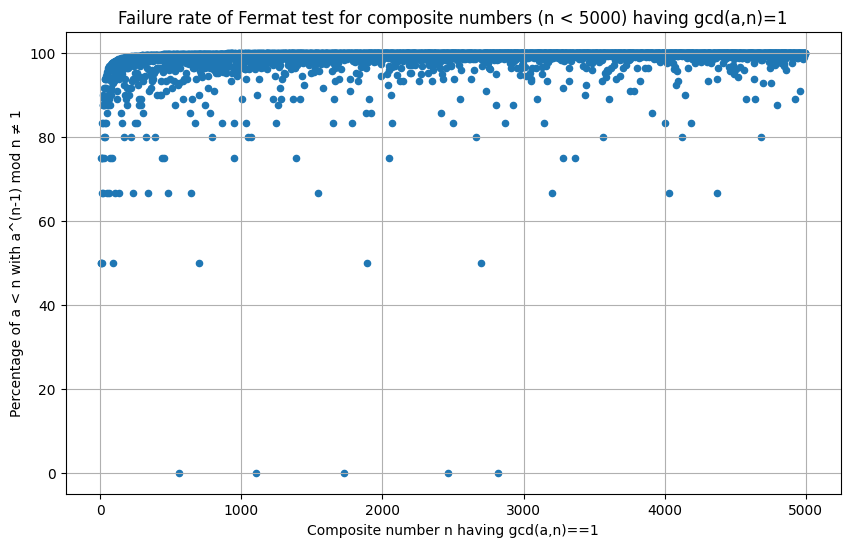
\includegraphics[width=\textwidth]{experiment_plots/failure_fermat_among_gcd(a,n)_1.png}
\caption*{Only coprime bases \(\gcd(a,n)=1\): Carmichael numbers appear as near-zero-failure outliers, while non-Carmichael composites stay at or above the \(50\%\) failure level.}
\end{minipage}
\caption{Experimental behavior of Fermat's test for composite numbers below \(5000\). The left plot measures failure among all bases \(a<n\), while the right plot measures failure only among coprime bases.}
\label{fig:fermat-experiments}
\end{figure}

Figure~\ref{fig:fermat-experiments} connects the proofs with direct experimentation. In the left plot, most composite numbers are rejected by Fermat's test for a large percentage of all bases, so the theorem is often useful in practice as a quick filter. The right plot is more informative mathematically because it restricts attention to coprime bases, the only bases that can possibly fool Fermat's congruence.

This second experiment matches the theoretical picture very well. For non-Carmichael composite numbers, once there exists one coprime witness, at least half of the coprime bases must be witnesses, so the failure percentage should be at least \(50\%\). The plot shows that behavior clearly. The exceptional near-zero-failure outliers are the Carmichael numbers, which explains why Fermat's test alone is not strong enough for reliable primality testing.

\subsection{Step 4: Why Fermat's test is still not enough}
Unfortunately, Fermat's test is not always reliable. There are composite numbers \(n\) for which
\[
a^{n-1}\equiv 1 \pmod{n}
\]
for every \(a\) with \(\gcd(a,n)=1\). Such numbers are called \emph{Carmichael numbers}. For them, Fermat's test gives no witness at all, even though the number is composite.

So the next idea is not to look only at the final value \(a^{n-1}\), but also at the intermediate repeated squarings that lead to it.

\subsection{Step 5: Decompose \texorpdfstring{$n-1$}{n-1} and inspect the repeated squaring chain}
Let \(n\) be an odd integer greater than \(2\). Write
\[
n-1=2^s d
\]
where \(d\) is odd.

For a chosen base \(a\), define the sequence
\[
x_0=a^d,\quad x_1=a^{2d},\quad x_2=a^{4d},\quad \dots,\quad x_s=a^{2^s d}
\pmod{n}.
\]
Notice that
\[
x_s=a^{n-1}\pmod{n}.
\]

If \(n\) is prime, then Fermat's Little Theorem gives
\[
x_s\equiv 1 \pmod{n}.
\]
Now suppose \(x_0\not\equiv 1 \pmod{n}\). Since the sequence ends at \(1\), there must be a first index \(j\ge 1\) such that
\[
x_j\equiv 1 \pmod{n}.
\]
Then
\[
x_{j-1}^2\equiv 1 \pmod{n}.
\]
For a prime modulus, the only square roots of \(1\) are \(1\) and \(-1\). Since \(j\) was chosen as the \emph{first} index with value \(1\), we know that \(x_{j-1}\not\equiv 1 \pmod{n}\). Therefore
\[
x_{j-1}\equiv -1 \pmod{n}.
\]

So for every prime \(n\), one of the following must happen:
\begin{itemize}
    \item \(a^d\equiv 1 \pmod{n}\), or
    \item for some \(0\le r<s\),
    \[
    a^{2^r d}\equiv -1 \pmod{n}.
    \]
\end{itemize}

This is exactly the condition behind the Miller-Rabin test. Any odd number that breaks this prime-only pattern is definitely composite.

The intuition is that Miller-Rabin does not trust only the final value \(a^{n-1}\bmod n\). Instead, it watches the whole repeated-squaring chain. For a prime modulus, the chain can reach \(1\) only in the ``safe'' way: either it starts at \(1\), or it reaches \(-1\) just before \(1\). If the chain reaches \(1\) from some other value, then we have found a nontrivial square root of \(1\), which cannot happen modulo an odd prime. That is the core reason the Miller-Rabin test is stronger than Fermat's test.

\chapter{The Miller-Rabin Primality Test}
\section{Algorithmic Idea}
Let \(n\) be an odd integer greater than \(2\), and let
\[
n - 1 = 2^s d
\]
with \(d\) odd. For a chosen base \(a\), the Miller-Rabin test computes
\[
x_0 = a^d \bmod n.
\]
If \(x_0 \equiv 1 \pmod{n}\) or \(x_0 \equiv -1 \pmod{n}\), the round is passed. Otherwise, the algorithm repeatedly squares:
\[
x_1 = x_0^2 \bmod n,\quad
x_2 = x_1^2 \bmod n,\quad \dots
\]
until it either finds \(-1 \bmod n\) or proves that \(n\) is composite.

The logic is simple:
\begin{itemize}
    \item if the expected prime-like pattern appears, the round passes;
    \item if the pattern is broken, the number is definitely composite.
\end{itemize}

\section{Simplified Pseudocode}
The version implemented in the project follows the standard Miller-Rabin structure:
\begin{enumerate}
    \item Handle small and even cases separately.
    \item Write \(n-1 = 2^s d\) with \(d\) odd.
    \item Choose a test base \(a\).
    \item Compute \(x = a^d \bmod n\).
    \item If \(x = 1\) or \(x = n-1\), accept this round.
    \item Otherwise square \(x\) up to \(s-1\) times modulo \(n\).
    \item If some squaring gives \(n-1\), accept this round.
    \item If none of them gives \(n-1\), declare \(n\) composite.
\end{enumerate}

In this repository, the implementation uses the fixed witness list
\[
\{2,3,5,7,11,13,17,19,23\}.
\]
This makes the behavior reproducible for experiments while preserving the basic Miller-Rabin logic.

\section{Simplified Correctness Proof for Prime Inputs}
We now prove the main property needed by the report: if \(n\) is an odd prime, then the Miller-Rabin test never incorrectly declares it composite.

\begin{lemma}
Let \(p\) be an odd prime. If
\[
x^2 \equiv 1 \pmod{p},
\]
then
\[
x \equiv 1 \pmod{p}
\quad \text{or} \quad
x \equiv -1 \pmod{p}.
\]
\end{lemma}

\begin{proof}
From \(x^2 \equiv 1 \pmod{p}\), we get
\[
x^2 - 1 \equiv 0 \pmod{p}.
\]
So
\[
(x-1)(x+1) \equiv 0 \pmod{p}.
\]
Because \(p\) is prime, it divides one of the two factors. Hence \(x \equiv 1 \pmod{p}\) or \(x \equiv -1 \pmod{p}\).
\end{proof}

\begin{theorem}
Let \(n\) be an odd prime and write
\[
n-1 = 2^s d
\]
with \(d\) odd. For every base \(a\) with \(1 < a < n\), either
\[
a^d \equiv 1 \pmod{n}
\]
or there exists an integer \(r\) with \(0 \le r < s\) such that
\[
a^{2^r d} \equiv -1 \pmod{n}.
\]
Therefore, a Miller-Rabin round cannot falsely reject a prime number.
\end{theorem}

\begin{proof}
Since \(n\) is prime and \(1 < a < n\), Fermat's Little Theorem gives
\[
a^{n-1} \equiv 1 \pmod{n}.
\]
Because \(n-1=2^s d\), define
\[
x_0 = a^d,\quad x_1 = a^{2d},\quad x_2 = a^{4d},\ \dots,\ x_s = a^{2^s d}
\pmod{n}.
\]
Then \(x_s \equiv a^{n-1} \equiv 1 \pmod{n}\).

If \(x_0 \equiv 1 \pmod{n}\), we are done. Otherwise, there must be some first index \(j\) such that
\[
x_j \equiv 1 \pmod{n}.
\]
Since \(x_j = x_{j-1}^2\), we have
\[
x_{j-1}^2 \equiv 1 \pmod{n}.
\]
By the lemma above, \(x_{j-1} \equiv 1 \pmod{n}\) or \(x_{j-1} \equiv -1 \pmod{n}\). But \(j\) was chosen as the first index giving \(1\), so \(x_{j-1} \not\equiv 1 \pmod{n}\). Hence
\[
x_{j-1} \equiv -1 \pmod{n}.
\]
Therefore some term in the sequence is \(-1 \bmod n\), exactly as Miller-Rabin expects for a prime input. So the algorithm cannot declare a prime number composite.
\end{proof}

\section{Why Composite Numbers Are Usually Detected Quickly}
For composite numbers, the Miller-Rabin conditions usually fail for many bases. Such bases are called \emph{witnesses} because they witness the compositeness of \(n\). In the randomized form of the algorithm, if bases are chosen independently and uniformly, the probability that a composite number passes one round is at most \(1/4\). After \(k\) independent rounds, the false-accept probability is at most
\[
\left(\frac{1}{4}\right)^k.
\]

The implementation in this project uses a fixed set of bases rather than random bases in each run. This gives deterministic and repeatable outputs for experiments. The theoretical \(4^{-k}\) statement belongs to the randomized version, but the fixed-basis implementation still performs very well in practice on the tested inputs.

\chapter{Other Algorithms in the Project}
\section{Square-Root Baseline}
The square-root method checks divisibility by integers up to \(\sqrt{n}\). It is exact and simple, which makes it a useful reference point. However, it becomes impractical very quickly as \(n\) grows.

\section{AKS Primality Test}
The AKS primality test was introduced by Agrawal, Kayal, and Saxena in their paper \textit{PRIMES is in P}. In this project, the AKS code implementation was written by ChatGPT. Its importance is mainly theoretical: it proves that primality testing can be done in deterministic polynomial time. In practice, however, AKS is much slower than Miller-Rabin for the input sizes considered in this project.

\section{Two Modular Reduction Strategies}
The repository includes two versions of modular multiplication inside Miller-Rabin:
\begin{itemize}
    \item \textbf{Ordinary modulo}: uses the usual division-based remainder path.
    \item \textbf{Fast modulo}: uses the custom \texttt{big\_int::fast\_mod} routine.
\end{itemize}

This is an important design choice because modular exponentiation dominates the runtime of Miller-Rabin. Improving the modular reduction step improves the overall test.

\chapter{Implementation Details}
\section{Core Arithmetic}
Large-number support is implemented through the custom \texttt{big\_int} class in \texttt{big\_int.cpp} and \texttt{big\_int.h}. The class provides:
\begin{itemize}
    \item construction from decimal and hexadecimal strings,
    \item comparison operations,
    \item addition, subtraction, multiplication, division, and remainder,
    \item halving and bit-length computation,
    \item a custom fast modular reduction function.
\end{itemize}

The class stores numbers in blocks of base \(10^9\), which simplifies decimal I/O while still supporting arbitrarily large inputs.

\section{Miller-Rabin Implementation}
The main Miller-Rabin logic appears in \texttt{miller\_rabin.cpp}. The implementation includes:
\begin{itemize}
    \item modular multiplication for ordinary and fast reduction,
    \item modular exponentiation by repeated squaring,
    \item primality testing using a fixed witness set,
    \item probable-prime generation for a requested bit length,
    \item previous-prime and next-prime search using Miller-Rabin.
\end{itemize}

Prime generation sets the highest and lowest bits so that the candidate has the requested bit length and is odd. Small-prime divisibility filters are applied before the Miller-Rabin test, reducing unnecessary full rounds.

\section{Console, Backend, and GUI}
The repository exposes the algorithms through multiple interfaces.
\begin{itemize}
    \item \texttt{main.cpp} provides a console application for decimal, hexadecimal, and dataset-based testing.
    \item \texttt{primality\_backend.cpp} provides a command-line backend that returns machine-readable key-value output.
    \item \texttt{primality\_gui.py} provides a Python Tkinter application for interactive checking and prime generation.
\end{itemize}

The GUI displays the results of ordinary Miller-Rabin, fast Miller-Rabin, and AKS together with timing information. It also reports the previous and next probable prime using fast Miller-Rabin.

\begin{figure}[htbp]
\centering
\begin{minipage}[t]{0.48\textwidth}
\centering
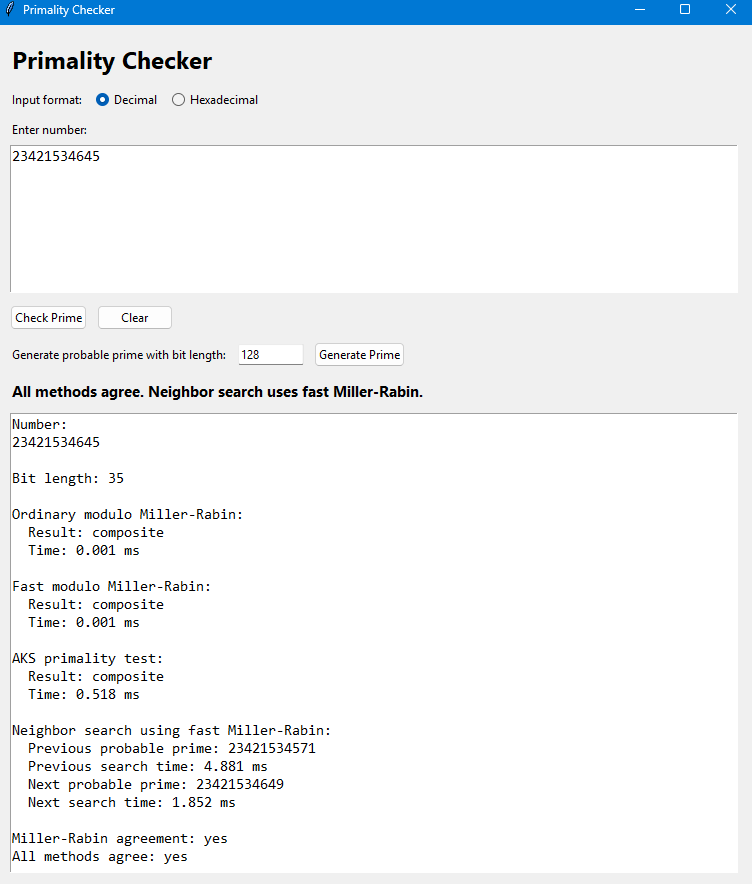
\includegraphics[width=\textwidth]{gui_pictures/gui_check_prime.png}
\caption*{Prime-checking view of the Tkinter GUI. The interface reports algorithm decisions, timings, and the previous and next probable prime around the queried input.}
\end{minipage}
\hfill
\begin{minipage}[t]{0.48\textwidth}
\centering
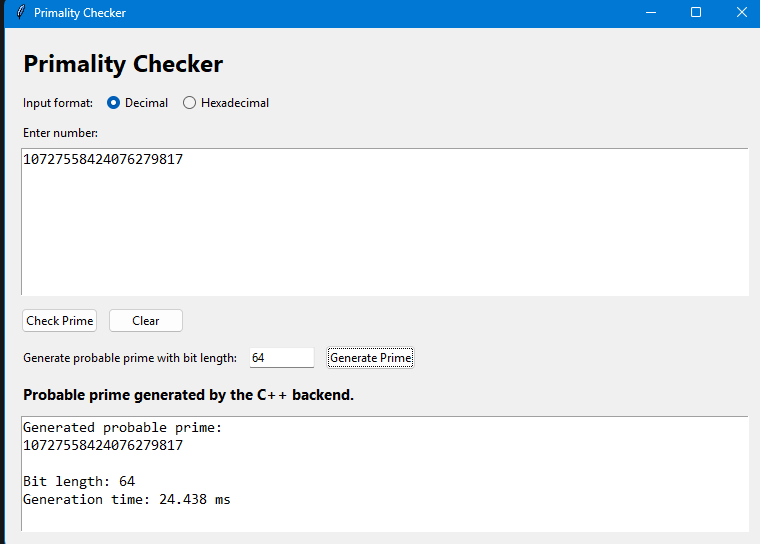
\includegraphics[width=\textwidth]{gui_pictures/gui_generate_image.png}
\caption*{Prime-generation view of the GUI. Users can request a target bit length and generate a probable prime interactively.}
\end{minipage}
\caption{Graphical interface provided by \texttt{primality\_gui.py}.}
\label{fig:gui-screens}
\end{figure}

Figure~\ref{fig:gui-screens} shows that the project is not limited to benchmark scripts or terminal commands. The interface makes the implemented algorithms usable for interactive demonstrations, quick testing, and prime generation during live presentation or classroom discussion.

\chapter{Experimental Evaluation}
\section{Bit-Length-Based Runtime Study}
The most meaningful way to compare primality-testing algorithms is by input bit length, not by the first few small primes. For that reason, the experimental discussion in this report uses bit-length-based runtime plots. These plots show how the algorithms behave as the size of the input grows, which is the quantity that actually drives their practical cost.

The AKS plots cover prime inputs from \(2\) to \(60\) bits, because the deterministic algorithm becomes very expensive beyond that range. The Miller-Rabin plots extend much further, up to \(4096\) bits, because the probabilistic test remains practical on much larger numbers. In the plots, scattered points represent measured samples and the smooth line represents the average trend.

\section{Individual Runtime Behavior}
\begin{figure}[htbp]
\centering
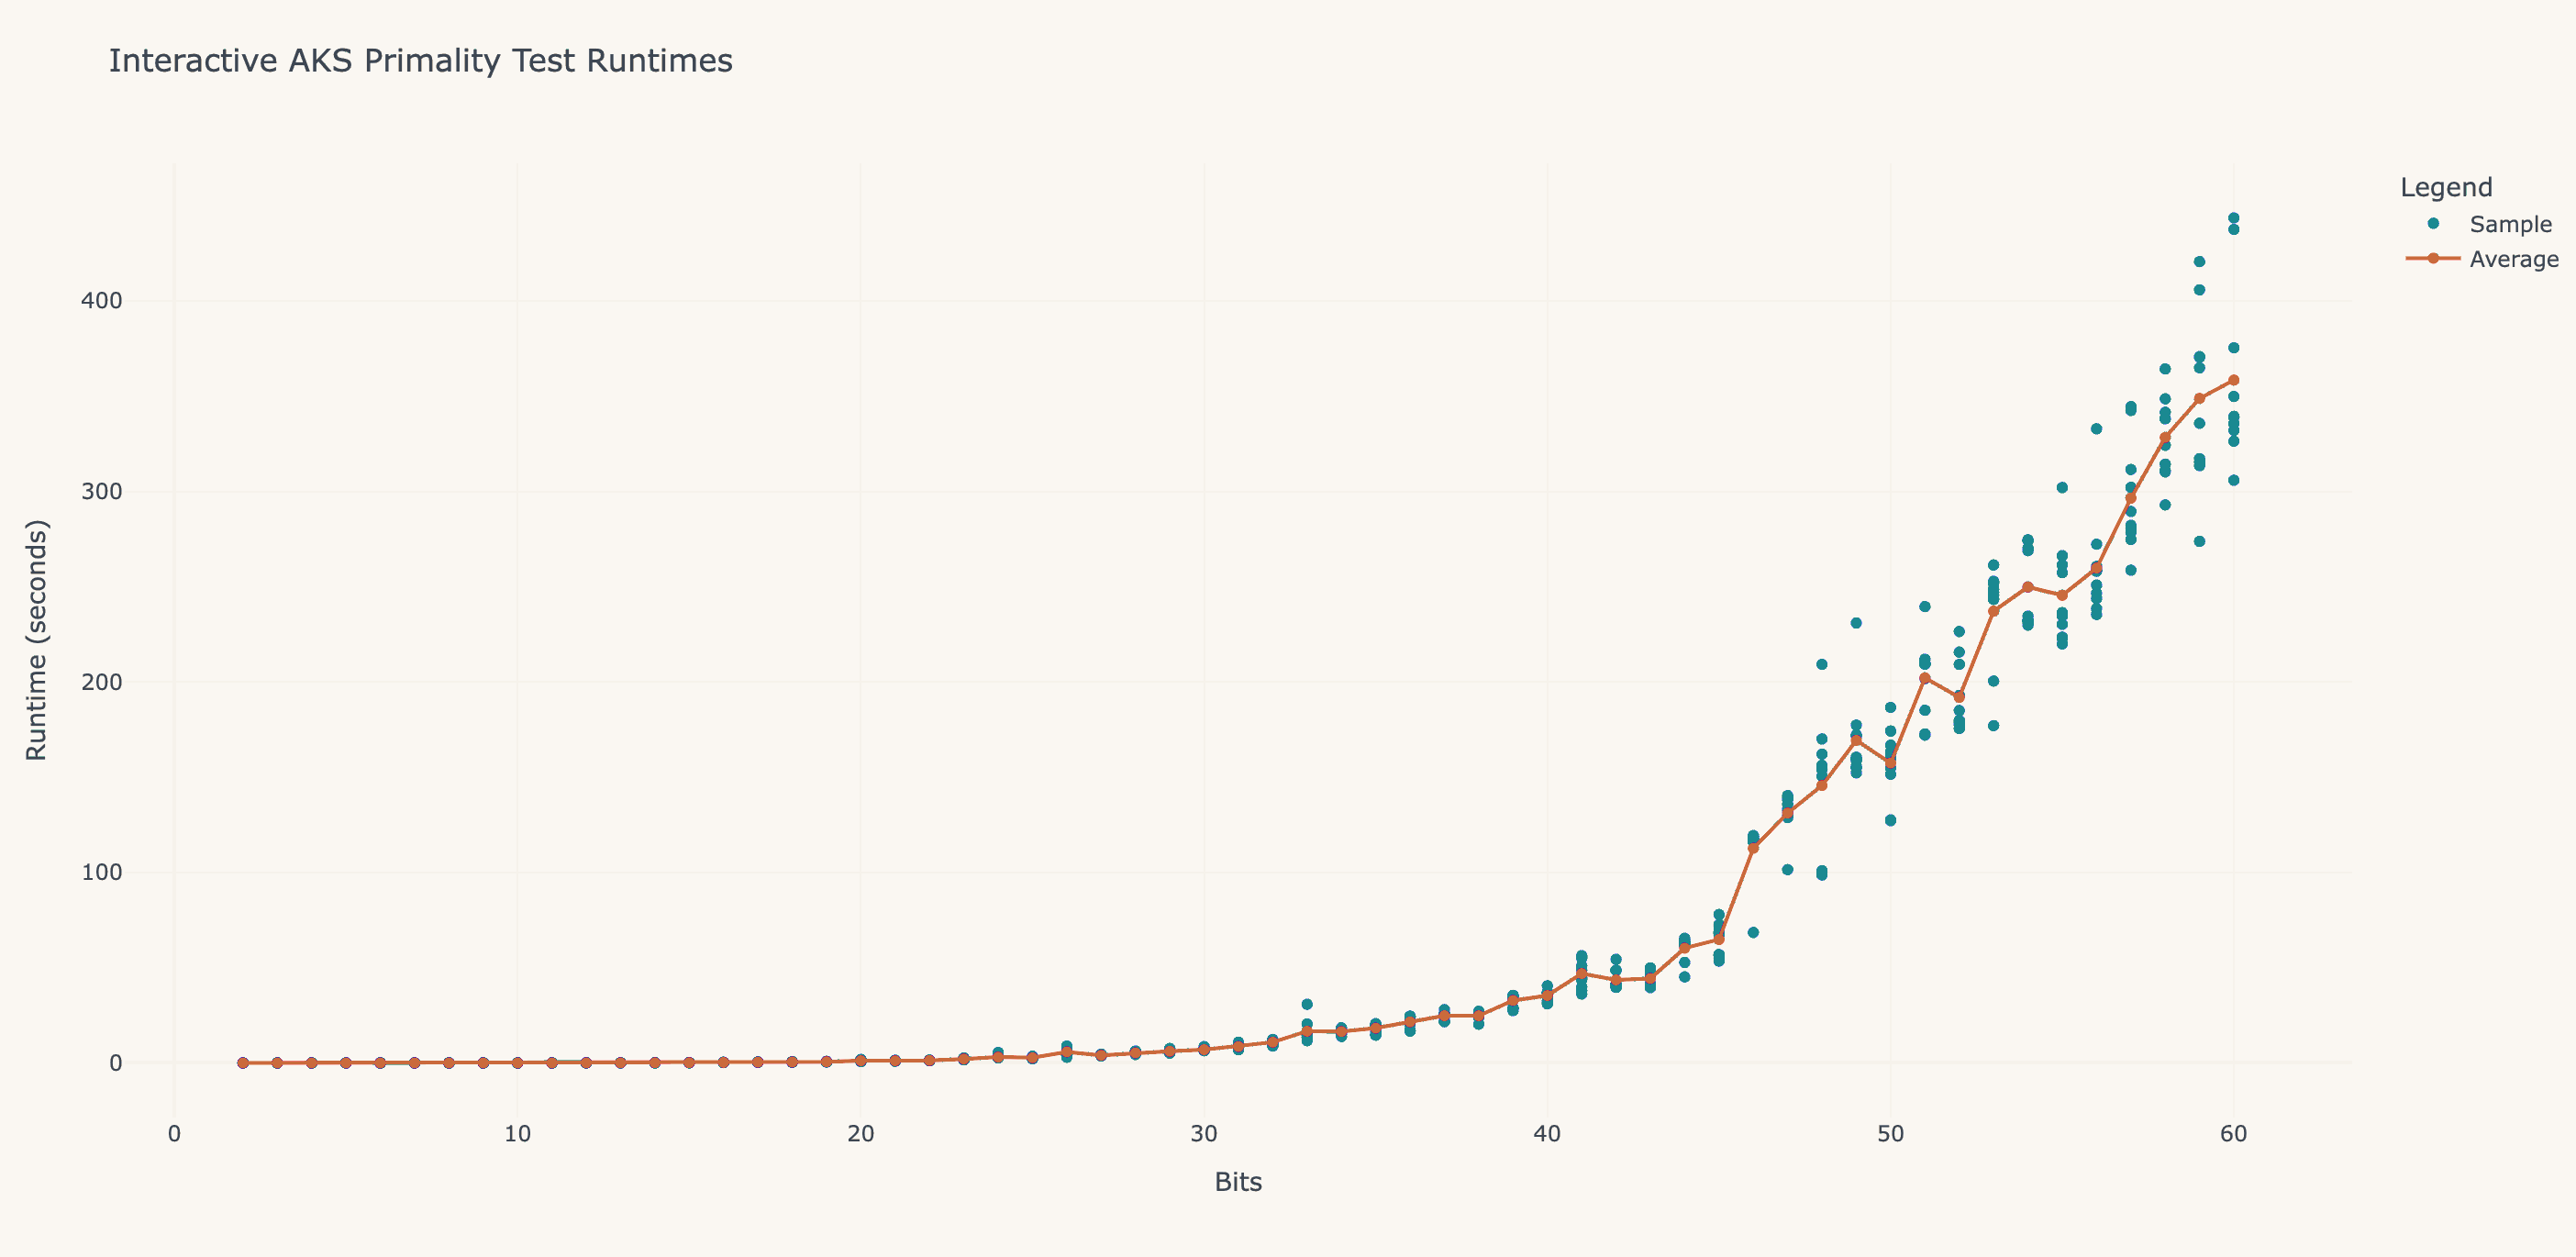
\includegraphics[width=0.88\textwidth]{images/aks_runtime_plot.png}
\caption{Runtime performance of the AKS algorithm for prime numbers of \(2\) to \(60\) bits. Each point represents a measured sample, and the red line indicates the average runtime.}
\label{fig:aks-runtime}
\end{figure}

\begin{figure}[htbp]
\centering
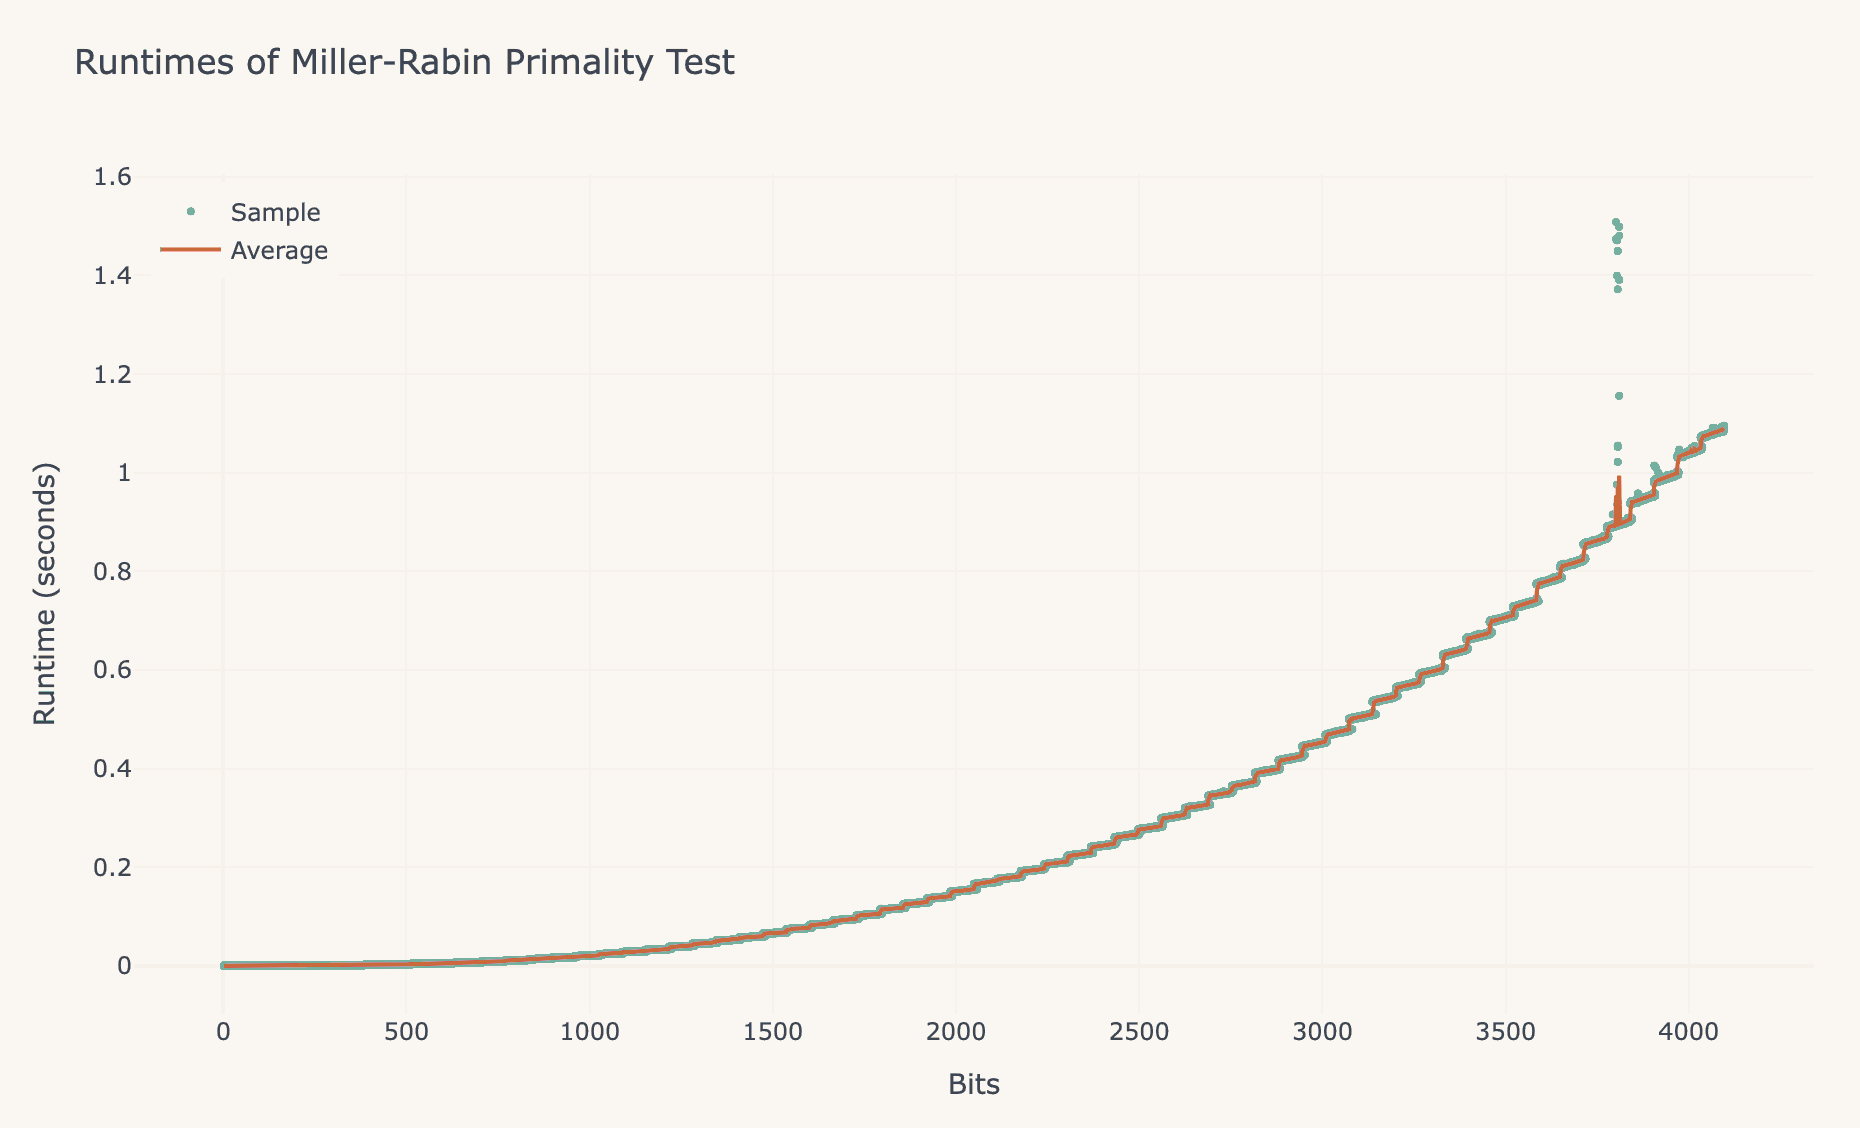
\includegraphics[width=0.82\textwidth]{images/miller_rabin_runtime_plot.png}
\caption{Runtime performance of the Miller-Rabin algorithm for prime numbers of \(2\) to \(4096\) bits. Each point represents a measured sample, and the red line indicates the average runtime.}
\label{fig:mr-runtime}
\end{figure}

Figures~\ref{fig:aks-runtime} and \ref{fig:mr-runtime} immediately show the main practical difference between the two algorithms. AKS grows sharply once the input size moves beyond the smaller bit-length range, while Miller-Rabin stays comparatively flat even when the bit length is increased all the way to \(4096\). This is exactly the pattern one expects from a deterministic but expensive method on one side and a highly efficient repeated modular-exponentiation test on the other.

\section{Direct Comparison on the Same Input Range}
\begin{figure}[htbp]
\centering
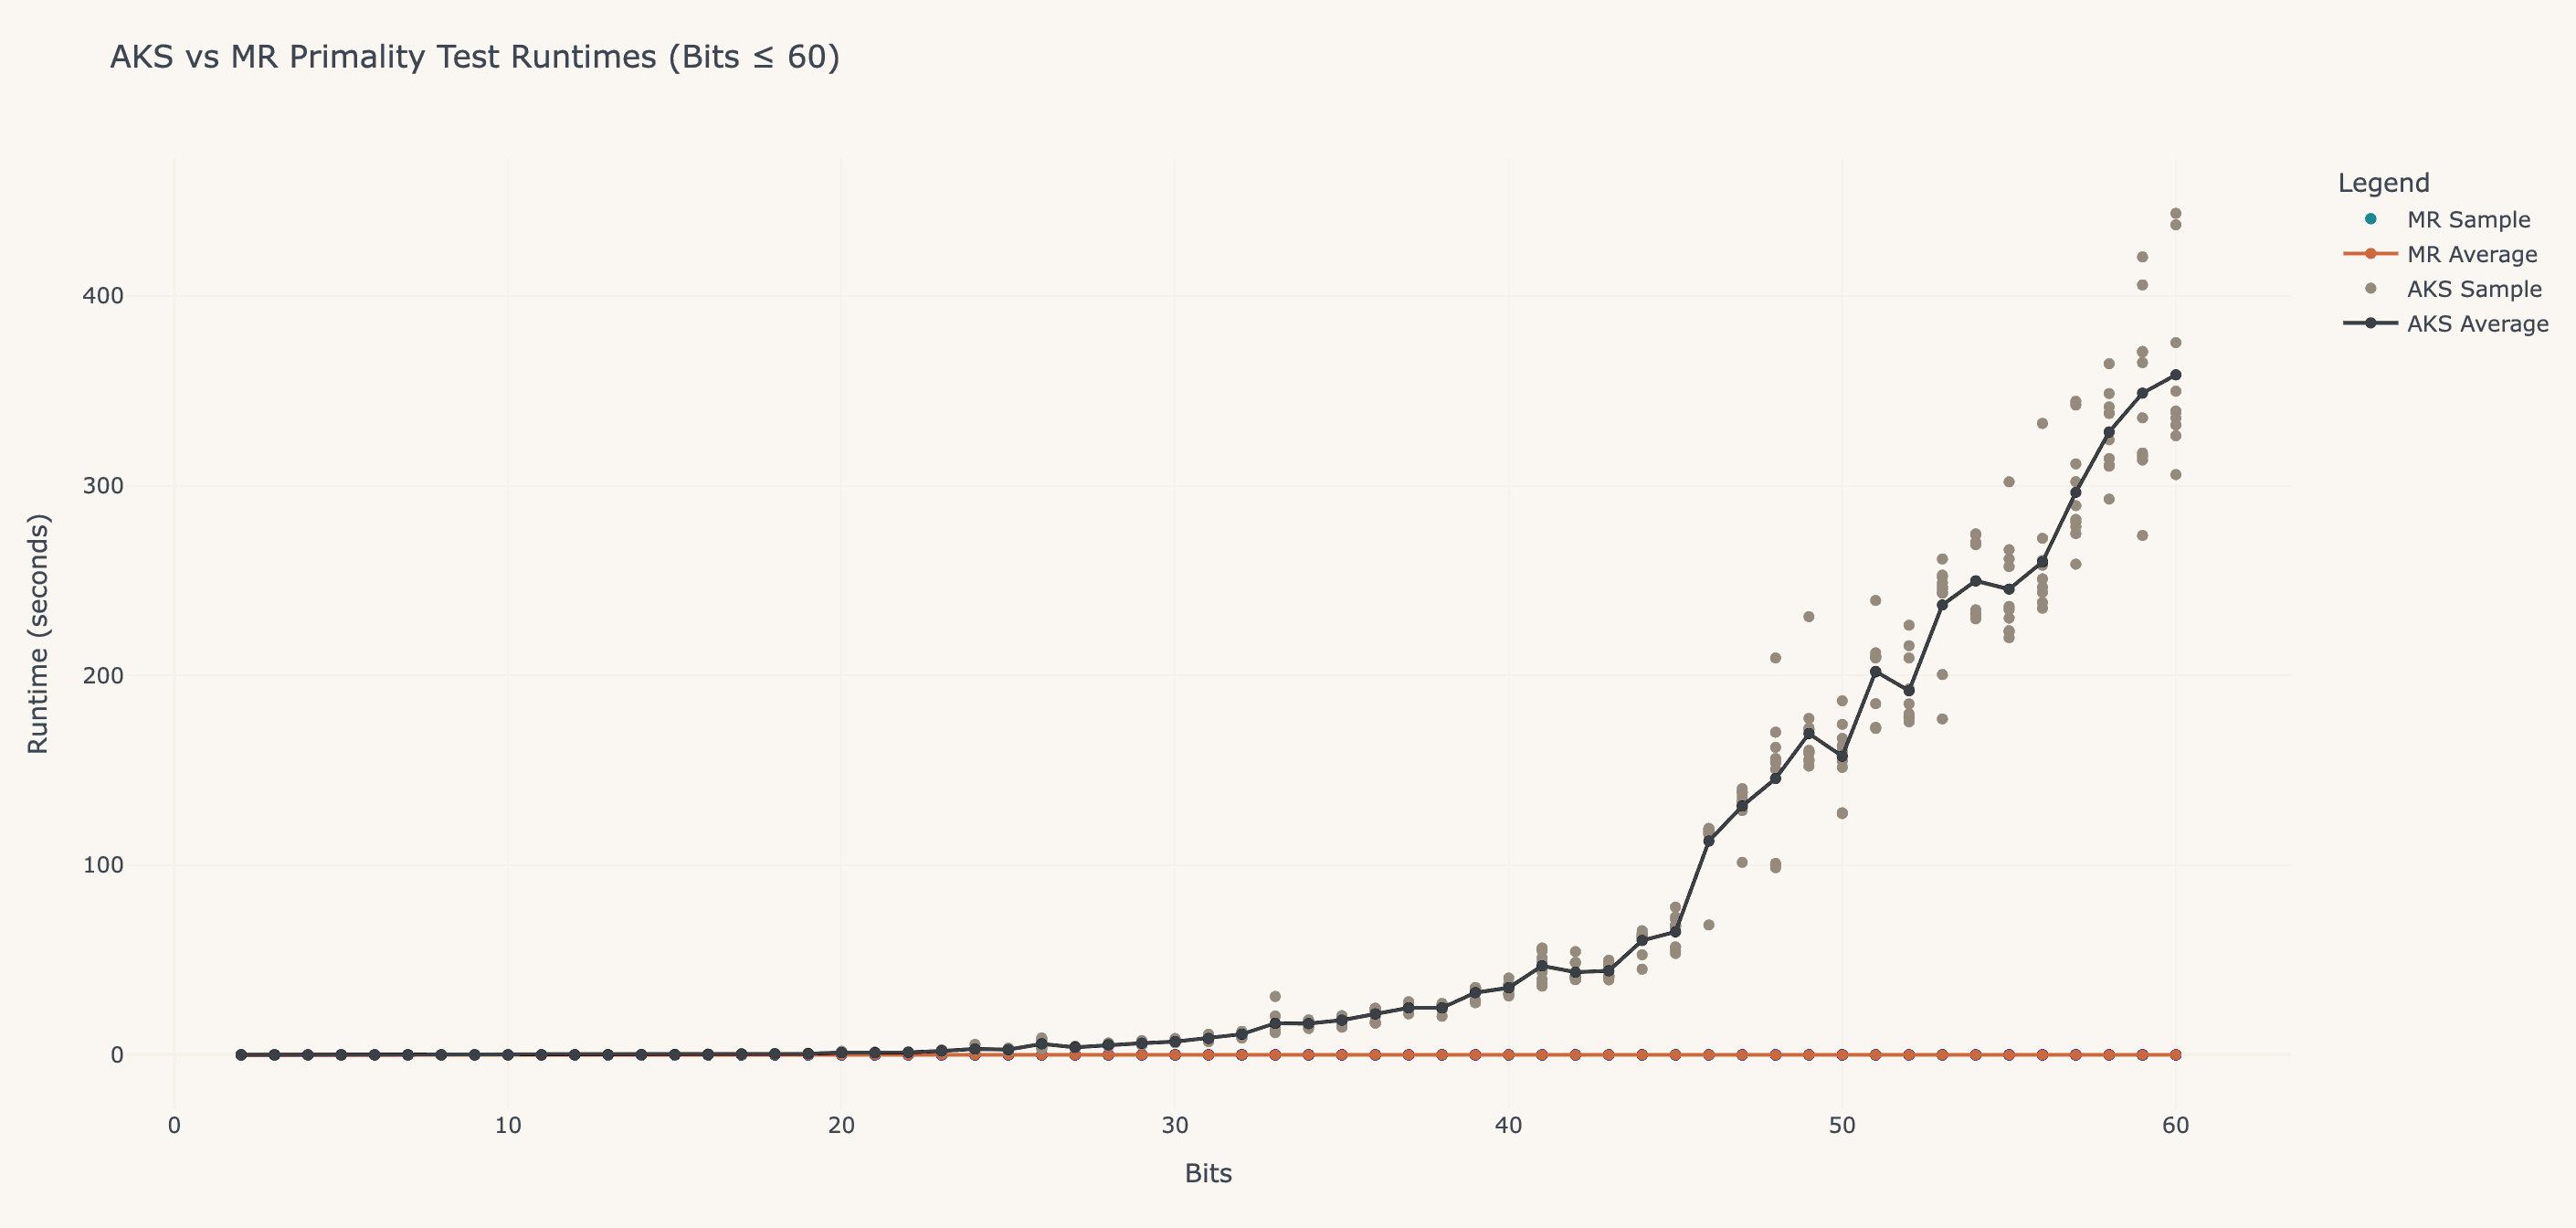
\includegraphics[width=0.88\textwidth]{images/aks_vs_miller_rabin_plot.png}
\caption{Comparison of runtime performance between AKS and Miller-Rabin for prime numbers of \(2\) to \(60\) bits.}
\label{fig:aks-mr-direct}
\end{figure}

\begin{figure}[htbp]
\centering
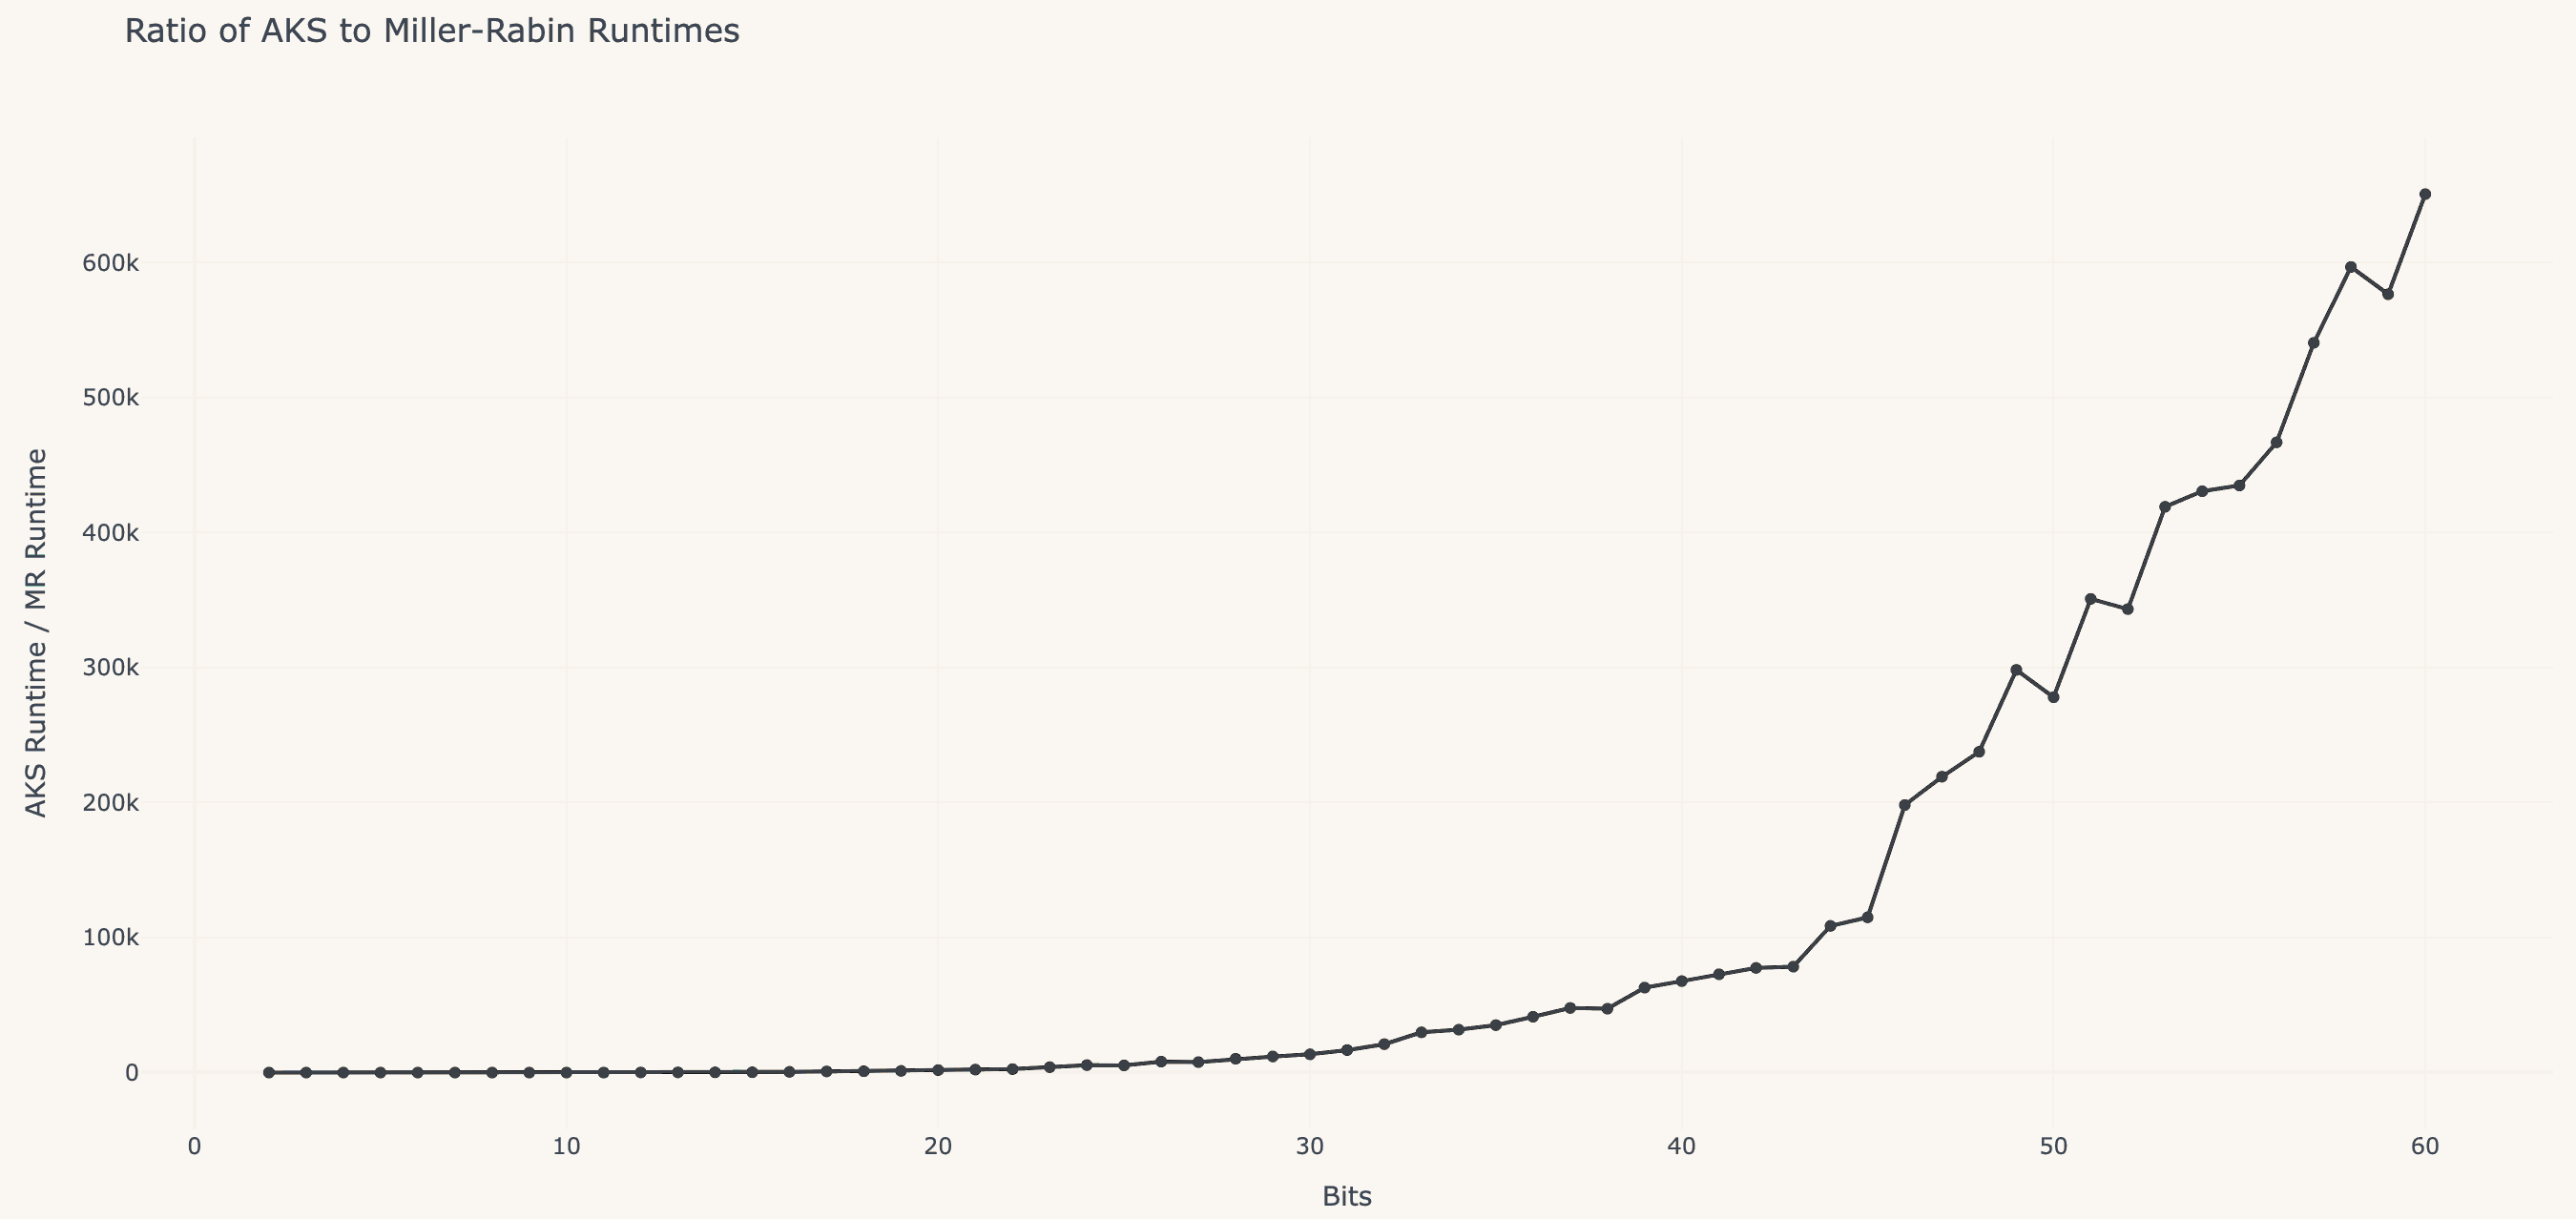
\includegraphics[width=0.88\textwidth]{images/aks_miller_rabin_ratio_plot.png}
\caption{Ratio of AKS average runtime to Miller-Rabin average runtime for prime numbers of \(2\) to \(60\) bits.}
\label{fig:aks-mr-ratio}
\end{figure}

Figure~\ref{fig:aks-mr-direct} shows both algorithms on the same horizontal range, so the gap is easy to see without changing scales. The Miller-Rabin measurements stay close to the baseline, whereas AKS rises rapidly with bit length. Figure~\ref{fig:aks-mr-ratio} quantifies the same gap more clearly: the runtime ratio keeps increasing and reaches the order of \(7\times 10^5\) by \(60\) bits. In other words, at that scale AKS is hundreds of thousands of times slower than Miller-Rabin on the tested prime inputs.

\section{Extended-Range Miller-Rabin View}
\begin{figure}[htbp]
\centering
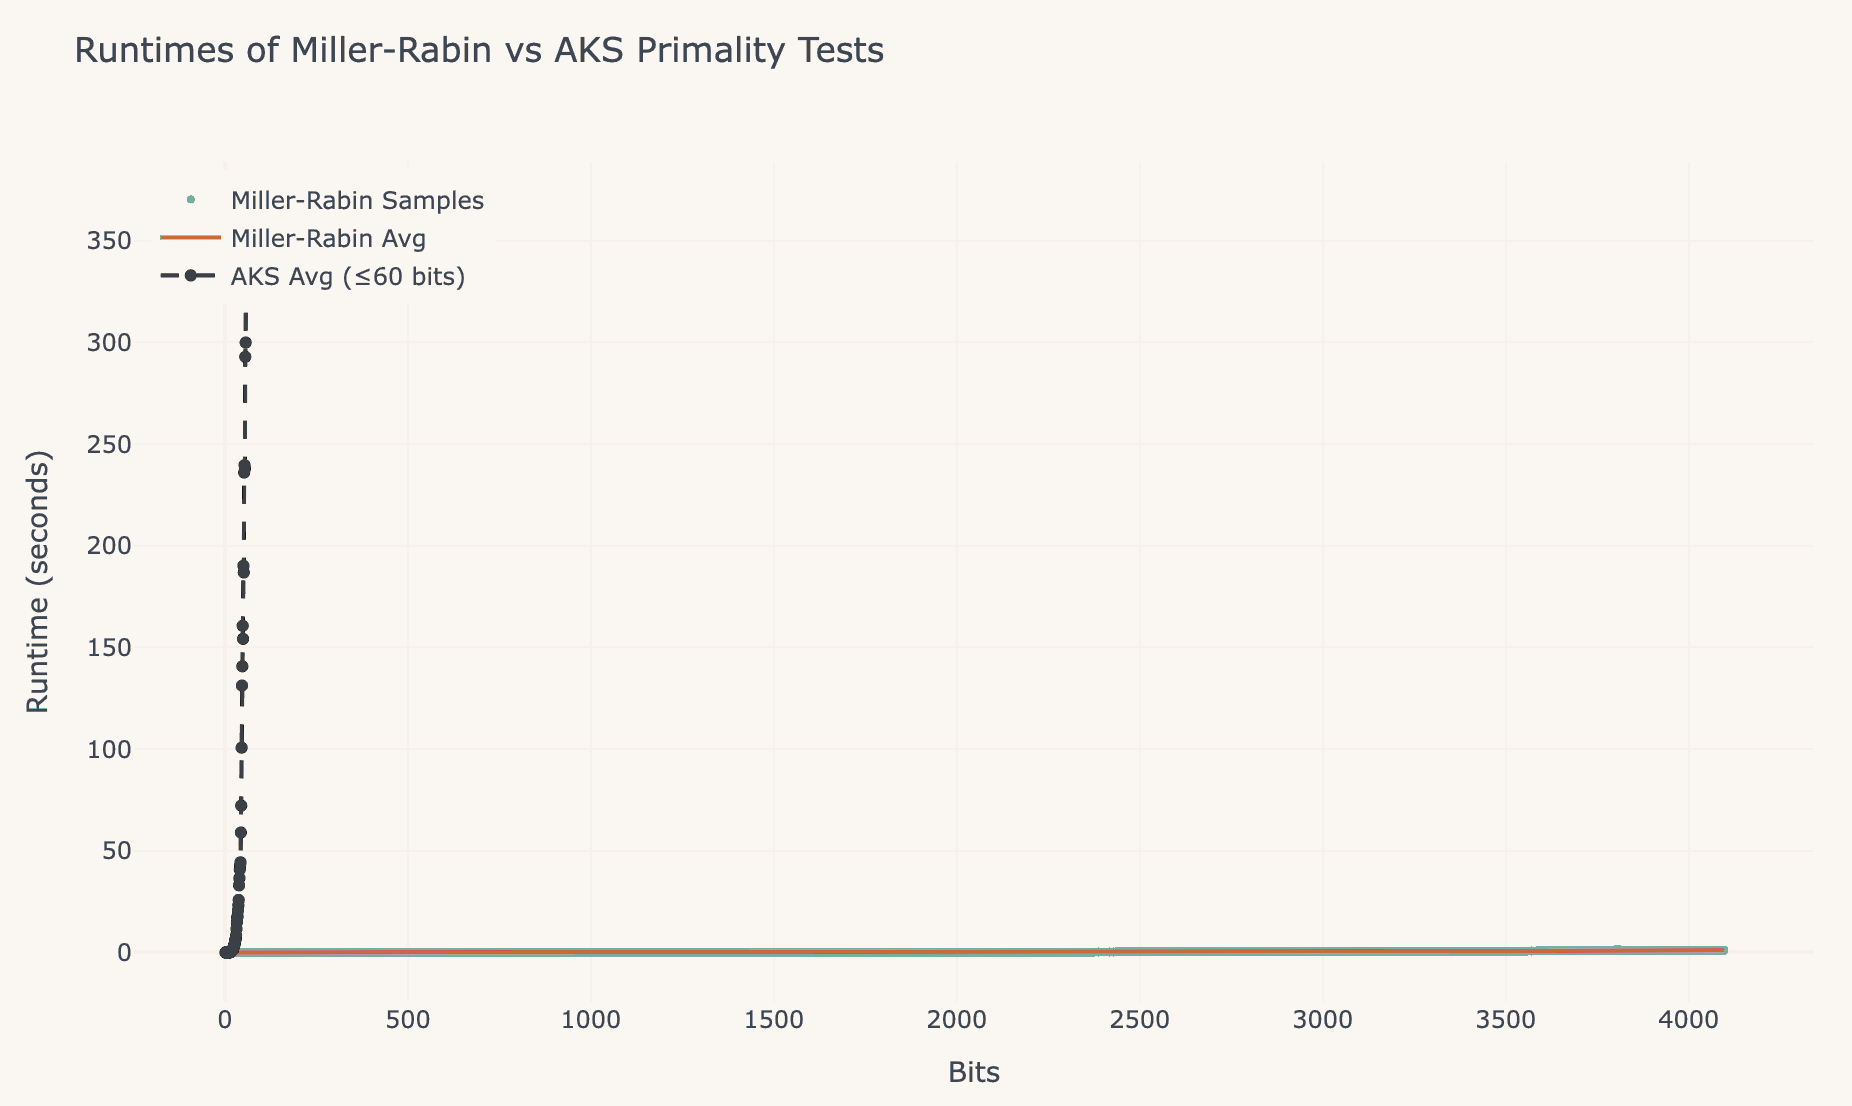
\includegraphics[width=0.82\textwidth]{images/aks_vs_miller_rabin_extended_plot.png}
\caption{Extended comparison showing AKS up to \(60\) bits and Miller-Rabin up to \(4096\) bits on the same graph.}
\label{fig:extended-comparison}
\end{figure}

The extended comparison in Figure~\ref{fig:extended-comparison} makes the practical story even clearer. AKS already reaches runtimes of several hundred seconds by only \(60\) bits, while Miller-Rabin continues far beyond that range and still stays in the low-second regime even at \(4096\) bits. This wide separation is exactly why Miller-Rabin is the method that remains useful when the input size becomes cryptographically relevant.

\section{Prime-Search Benchmark by Bit Length}
The direct primality-test plots above show how long it takes to check a single input. A second benchmark in the project asks a different practical question: how much time does it take to \emph{find} a prime of a given bit length? This is useful because many applications do not test one hand-picked number; they search upward through candidates until a prime is found.

For this benchmark, the code starts from the smallest number of each bit length and searches upward until it finds the first prime. The comparison covers bit lengths \(1\) through \(200\). Miller-Rabin is run through the full range, while the square-root method is stopped once a single bit length exceeds a two-second cap, because beyond that point the exact baseline becomes too slow to remain informative.

\begin{figure}[htbp]
\centering
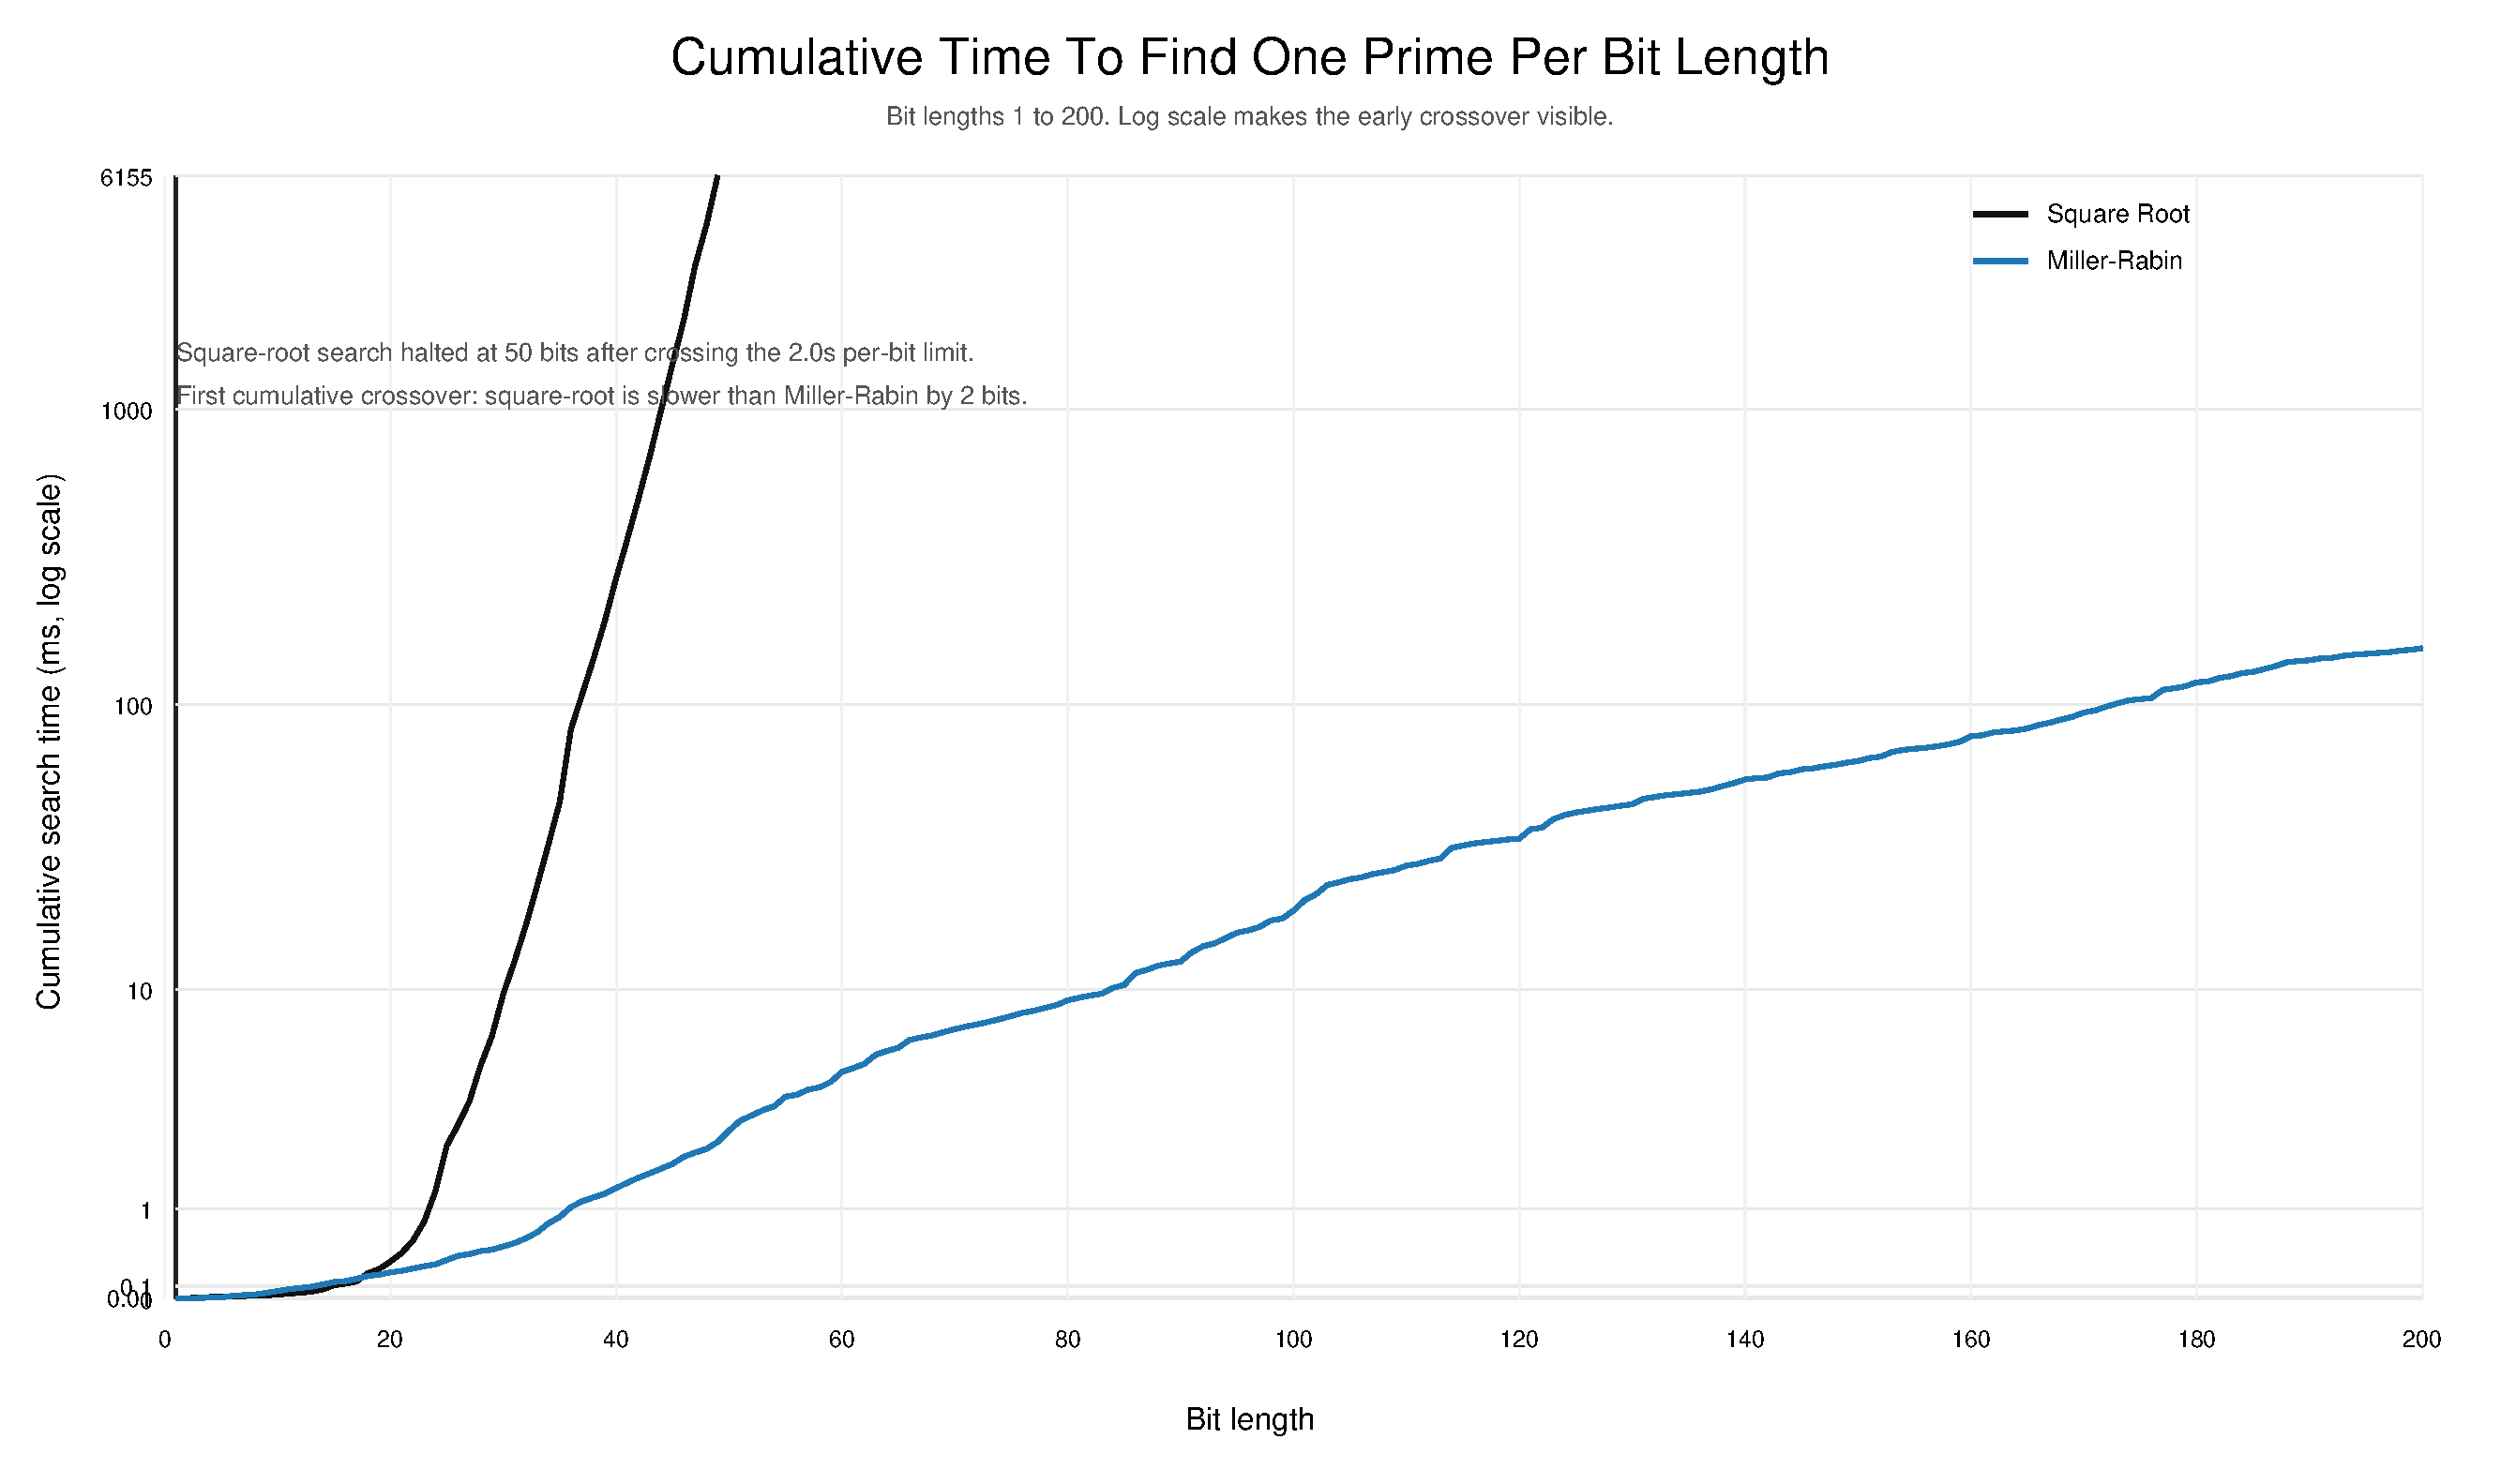
\includegraphics[width=0.86\textwidth]{images/bit_length_prime_search_comparison_log.pdf}
\caption{Log-scale cumulative comparison of the time required to find one prime for each bit length from \(1\) to \(200\). The square-root search is stopped once the per-bit cap is exceeded.}
\label{fig:bit-search-log}
\end{figure}

Figure~\ref{fig:bit-search-log} makes the practical gap especially clear. The square-root search hits the two-second per-bit cap at \(50\) bits, and its cumulative time is already about \(6155.79\) ms by \(49\) bits. Miller-Rabin, by contrast, completes the entire \(1\)-to-\(200\)-bit run with only about \(155.41\) ms of cumulative search time. This benchmark reinforces the same conclusion as the direct runtime plots: exact naive methods become unusable quickly, whereas Miller-Rabin remains efficient even when the task is not just checking one number but actually finding primes across increasing bit lengths.

\section{Ordinary Modulo vs Fast Modulo Inside Miller-Rabin}
The project also benchmarks the two Miller-Rabin arithmetic paths against each other. This comparison is narrower than the AKS-versus-Miller-Rabin plots, because both methods use the same primality logic. The purpose here is to measure whether the custom fast modular reduction routine improves cumulative runtime in practice.

\begin{figure}[htbp]
\centering
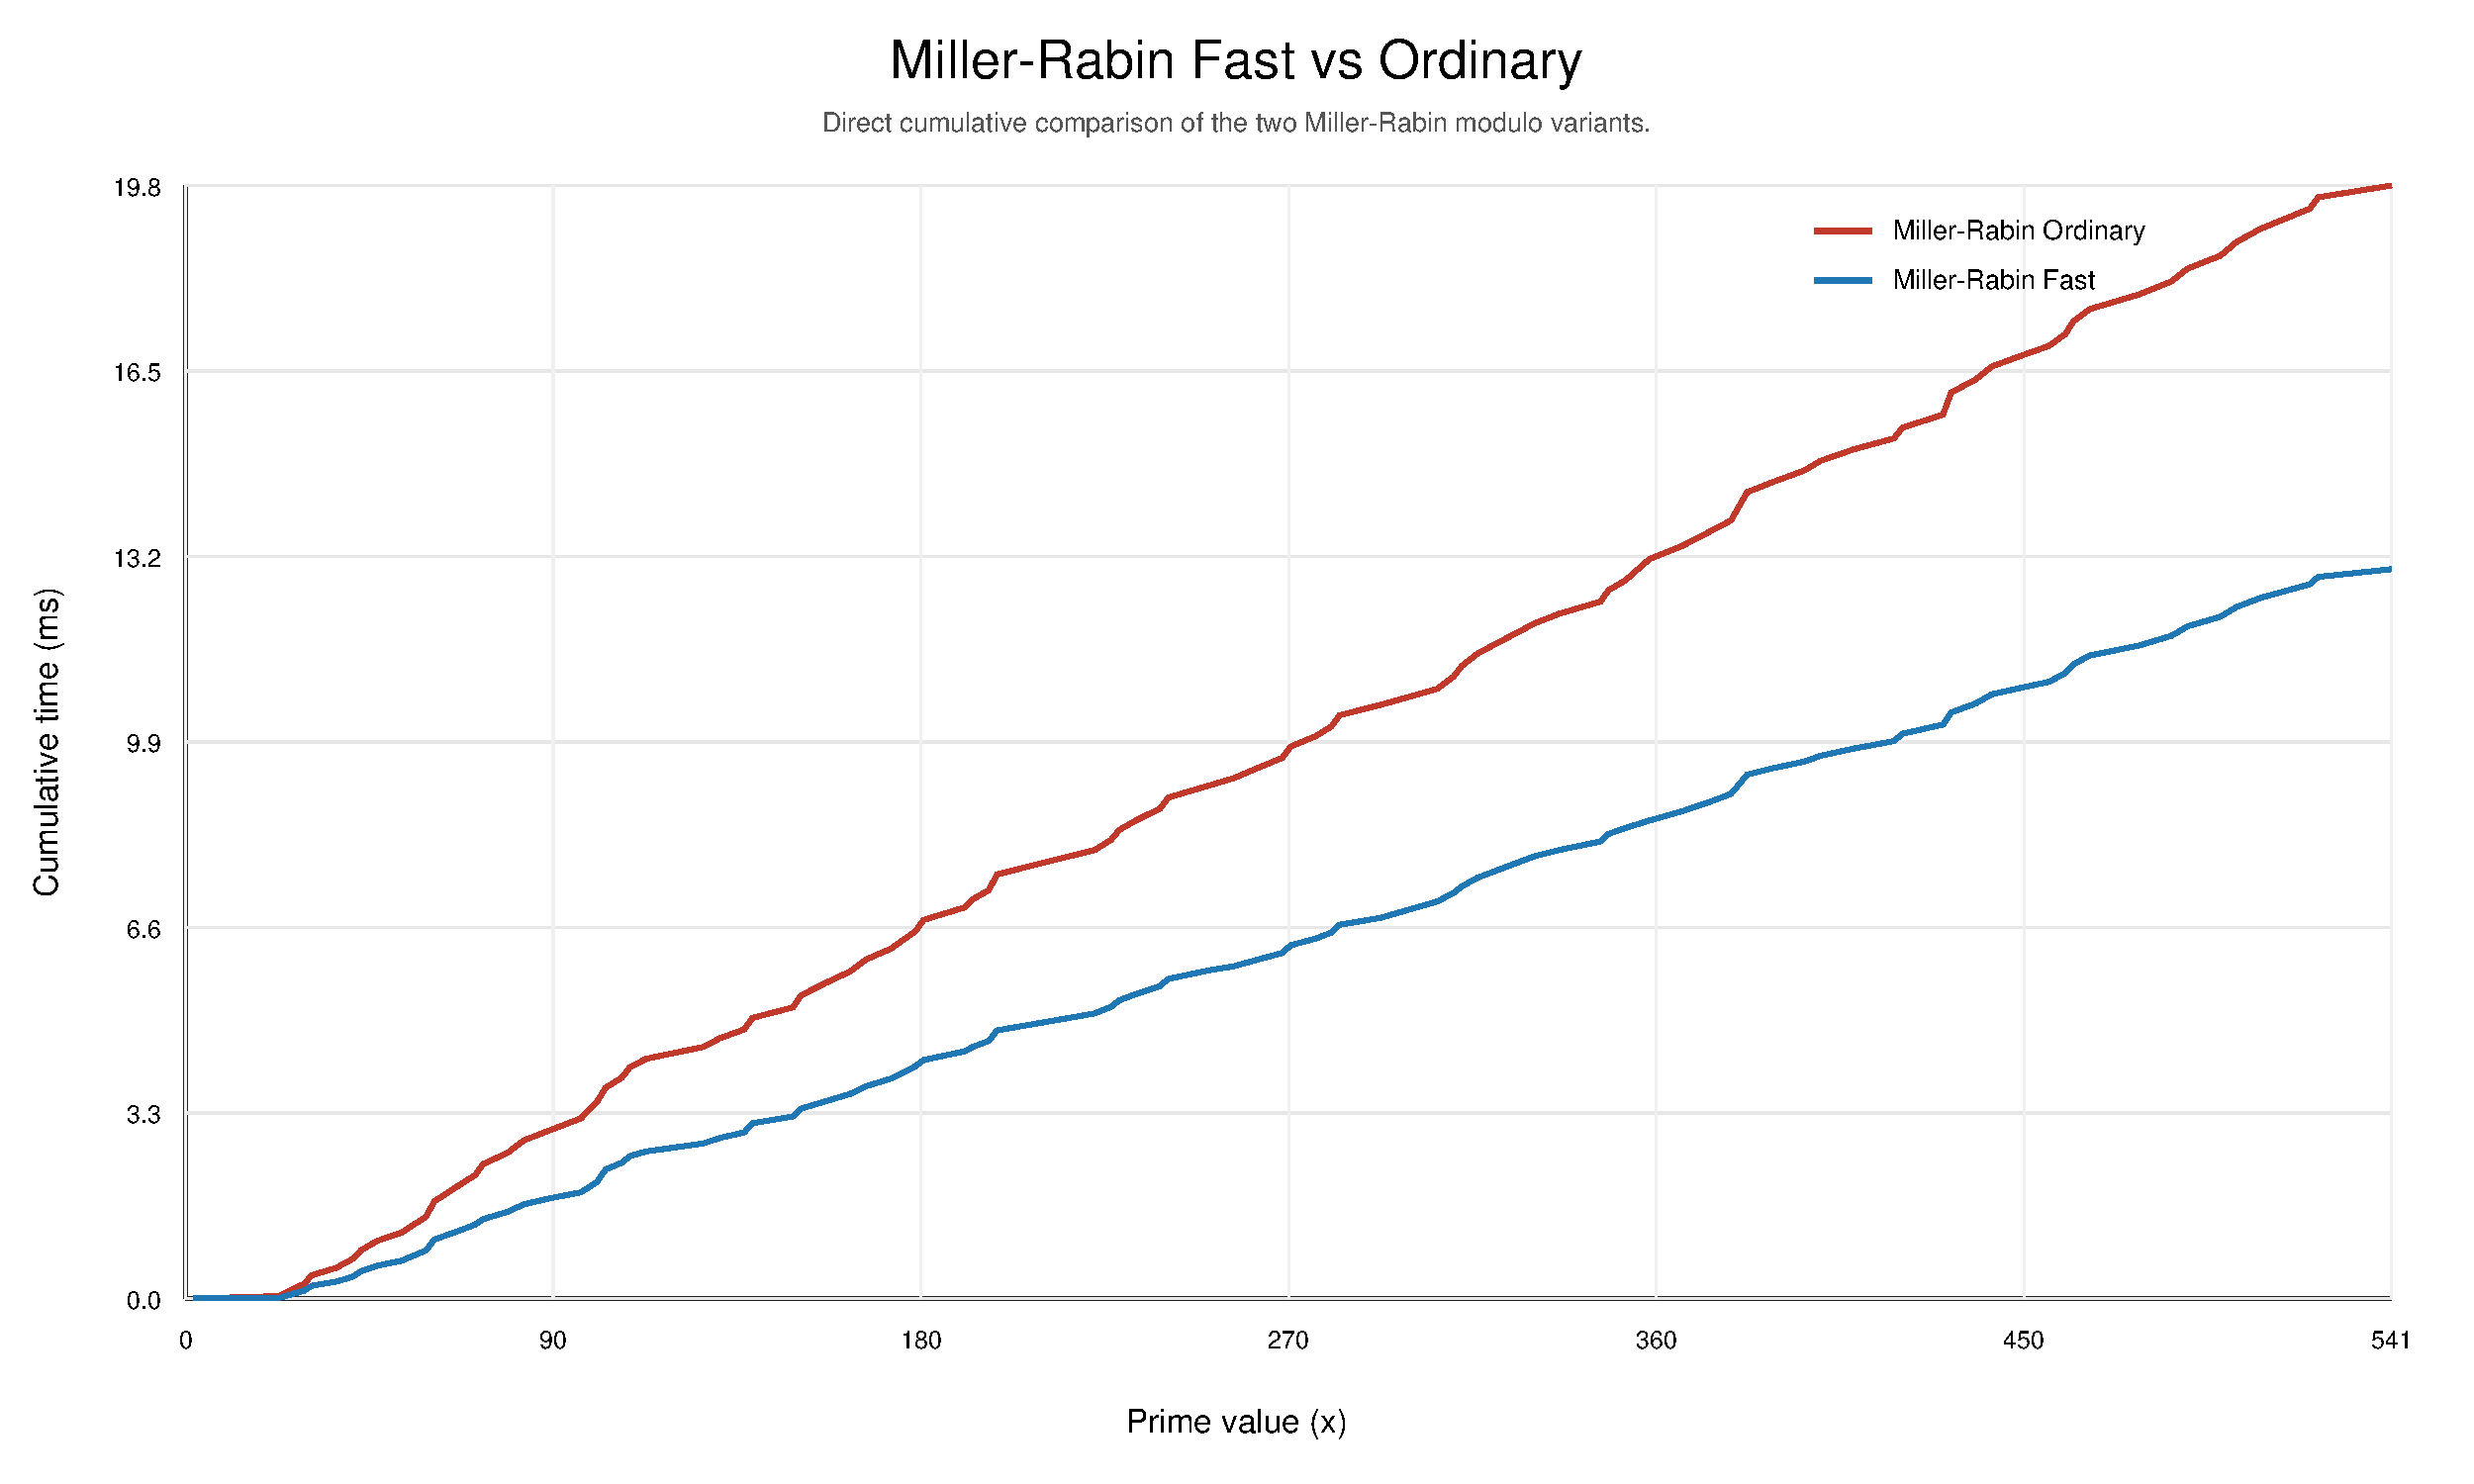
\includegraphics[width=0.78\textwidth]{images/miller_rabin_fast_vs_ordinary.pdf}
\caption{Cumulative comparison of Miller-Rabin using ordinary modulo versus the custom fast modulo reduction path.}
\label{fig:mr-fast-ordinary}
\end{figure}

Figure~\ref{fig:mr-fast-ordinary} shows that the fast modular reduction path consistently stays below the ordinary modulo path in cumulative time. In the generated benchmark CSV, the cumulative ordinary-modulo time is about \(19.77\) ms, whereas the fast-modulo version finishes in about \(12.95\) ms on the same data, a ratio of roughly \(1.53\) in favor of the fast path. This does not change the high-level conclusion that Miller-Rabin is the most practical algorithm in the project, but it does show that low-level arithmetic implementation choices still matter for total runtime.

\section{Discussion}
Taken together, these benchmark families tell a consistent story. AKS is mathematically important because it gives a deterministic polynomial-time test, but its runtime grows too quickly for large inputs. The square-root baseline is exact and useful for intuition, yet its prime-search cost becomes impractical even at moderate bit lengths. Miller-Rabin, by contrast, stays fast over a much larger range and is therefore the more practical choice for real computation, especially in cryptographic settings. The internal ordinary-versus-fast-modulo comparison further shows that implementation details inside Miller-Rabin can still produce measurable runtime gains.

\chapter{Conclusion}
This project demonstrates that primality testing is a good example of the difference between theoretical possibility and practical efficiency. The square-root method is mathematically straightforward but scales poorly. AKS provides deterministic polynomial-time correctness but becomes expensive very quickly in practice. Miller-Rabin, on the other hand, offers an excellent engineering trade-off: its mathematical structure is strong enough to avoid the weaknesses of basic Fermat-style testing, and its runtime remains low for much larger inputs.

The report also shows that implementation and algorithmic choices matter. A theoretically strong method is not automatically the most useful one in practice, and the surrounding software design makes the algorithms easier to test, compare, and use interactively. Overall, the repository successfully combines theory, proof, implementation, experimentation, and user-facing tooling in one coherent primality-testing project.

\section*{References Used}
\begin{itemize}
    \item M. Agrawal, N. Kayal, and N. Saxena, \textit{PRIMES is in P}, Annals of Mathematics, 160(2), 781--793, 2004.
    \item G. L. Miller, \textit{Riemann's Hypothesis and Tests for Primality}, Journal of Computer and System Sciences, 1976.
    \item M. O. Rabin, \textit{Probabilistic Algorithm for Testing Primality}, Journal of Number Theory, 1980.
    \item OpenAI, \textit{ChatGPT}, used to write the AKS code implementation for this project, accessed April 5, 2026.
\end{itemize}

\end{document}
